\documentclass[UTF8]{ctexart}
\usepackage{geometry}
\usepackage{indentfirst}
\usepackage{hyperref}
\usepackage{harpoon}
\usepackage{amsmath}
\usepackage{amssymb}
\usepackage{graphicx}
\usepackage{float}
\usepackage{subfigure}
\usepackage{multirow}
\usepackage{array}
\usepackage{tikz}
\usetikzlibrary{arrows, shapes, positioning, calc}
\geometry{a4paper, left=1cm, right=1cm, top=2cm, bottom=2cm}
\setlength{\parindent}{1cm}
\renewcommand\contentsname{Content}
\title{电阻网络}
\author{段元兴}
\date{\today}
\begin{document}
\maketitle
\thispagestyle{empty}
\setcounter{page}{1}
\newpage
\tableofcontents
\newpage
    \section{纯电阻网络}
        \subsection{计算结果与耗时}
            \begin{table}[H]
                \centering
                \caption{纯电阻网络阻值}
                \begin{tabular}{|c|c|c|c|c|c|}
                    \hline
                    规模&方法&正方形网络对角&正方形网络邻角&三角形网络&六边形网络\\
                    \hline
                    \multirow{2}*{1}&
                    分解法&1.000000000000&0.750000000000&0.666666666667&-\\
                    \cline{2-6}&
                    迭代法&1.000000000000&0.750000000000&0.666666666667&-\\
                    \hline
                    \multirow{2}*{4}&
                    分解法&2.136363636364&1.901515151515&1.674796747967&2.819373942470\\
                    \cline{2-6}&
                    迭代法&2.136363636364&1.901515151515&1.674796747967&2.819373942470\\
                    \hline
                    \multirow{2}*{16}&
                    分解法&3.685592463431&3.463587937288&3.024372524685&6.534376528387\\
                    \cline{2-6}&
                    迭代法&3.685592463431&3.463587937288&3.024372524685&6.534376528387\\
                    \hline
                    \multirow{2}*{64}&
                    分解法&5.392376786288&5.171646779480&4.503230022408&10.835436744804\\
                    \cline{2-6}&
                    迭代法&5.392376786288&5.171646779479&4.503230022408&10.835436744804\\
                    \hline
                    \multirow{2}*{256}&
                    分解法&7.142626030195&6.921984387704&6.019041361975&15.345275264273\\
                    \cline{2-6}&
                    迭代法&7.142626030199&6.921984387707&6.019041361975&15.345275264276\\
                    \hline
                    \multirow{2}*{1024}&
                    分解法&8.903985943880&8.683349963979&7.544427062276&19.911812607921\\
                    \cline{2-6}&
                    迭代法&8.903985944525&8.683349964498&7.544427062273&19.911812607780\\
                    \hline
                \end{tabular}
            \end{table}
            \begin{table}[H]
                \centering
                \caption{耗时(CPU: Ryzen 2700x, 单线程, 仅含解方程的时间, 单位: ms)}
                \begin{tabular}{|c|c|c|c|c|c|}
                    \hline
                    规模&方法&正方形网络对角&正方形网络邻角&三角形网络&六边形网络\\
                    \hline
                    \multirow{2}*{1}&
                    分解法&0.016&0.002&0.003&--\\
                    \cline{2-6}&
                    迭代法&0.053&0.054&1.392&--\\
                    \hline
                    \multirow{2}*{4}&
                    分解法&0.009&0.005&0.005&0.005\\
                    \cline{2-6}&
                    迭代法&0.058&0.062&3.172&0.410\\
                    \hline
                    \multirow{2}*{16}&
                    分解法&0.123&0.116&0.056&0.057\\
                    \cline{2-6}&
                    迭代法&0.511&0.509&1.001&0.415\\
                    \hline
                    \multirow{2}*{64}&
                    分解法&6.567&6.530&3.421&3.265\\
                    \cline{2-6}&
                    迭代法&22.500&24.670&12.120&11.517\\
                    \hline
                    \multirow{2}*{256}&
                    分解法&847.316&848.127&417.046&422.223\\
                    \cline{2-6}&
                    迭代法&1392.536&1813.554&716.513&754.238\\
                    \hline
                    \multirow{2}*{1024}&
                    分解法&204815.786&196280.548&98058.678&97958.859\\
                    \cline{2-6}&
                    迭代法&113630.867&128660.263&51435.261&54972.338\\
                    \hline
                \end{tabular}
            \end{table}
        \subsection{直接解法-带状对称矩阵Cholesky分解法}
            \indent 这里使用了带状对称矩阵的Cholesky分解法, 构造完带状矩阵之后直接分解然后求解2个
            三角方程组即可.%而由于直接的连续存储带状矩阵的方式
        \subsection{迭代解法-稀疏矩阵共轭梯度迭代法}
            \indent 由于构造出来的矩阵是稀疏的 (每行只有几个元素非零), 所以在使用迭代法的时候, 采用
            稀疏矩阵 (对使用带状矩阵也进行过测试, 得到的耗时是稀疏矩阵的几倍).
        \subsection{耗时比较}
            \indent 发现$O(n^3)$的直接解法的常数因子比迭代法小很多, 但是在大约512的规模下, 迭代法已经比直接解法快了.
    \section{交流网络}
        \subsection{计算结果与耗时}
            \begin{center}
                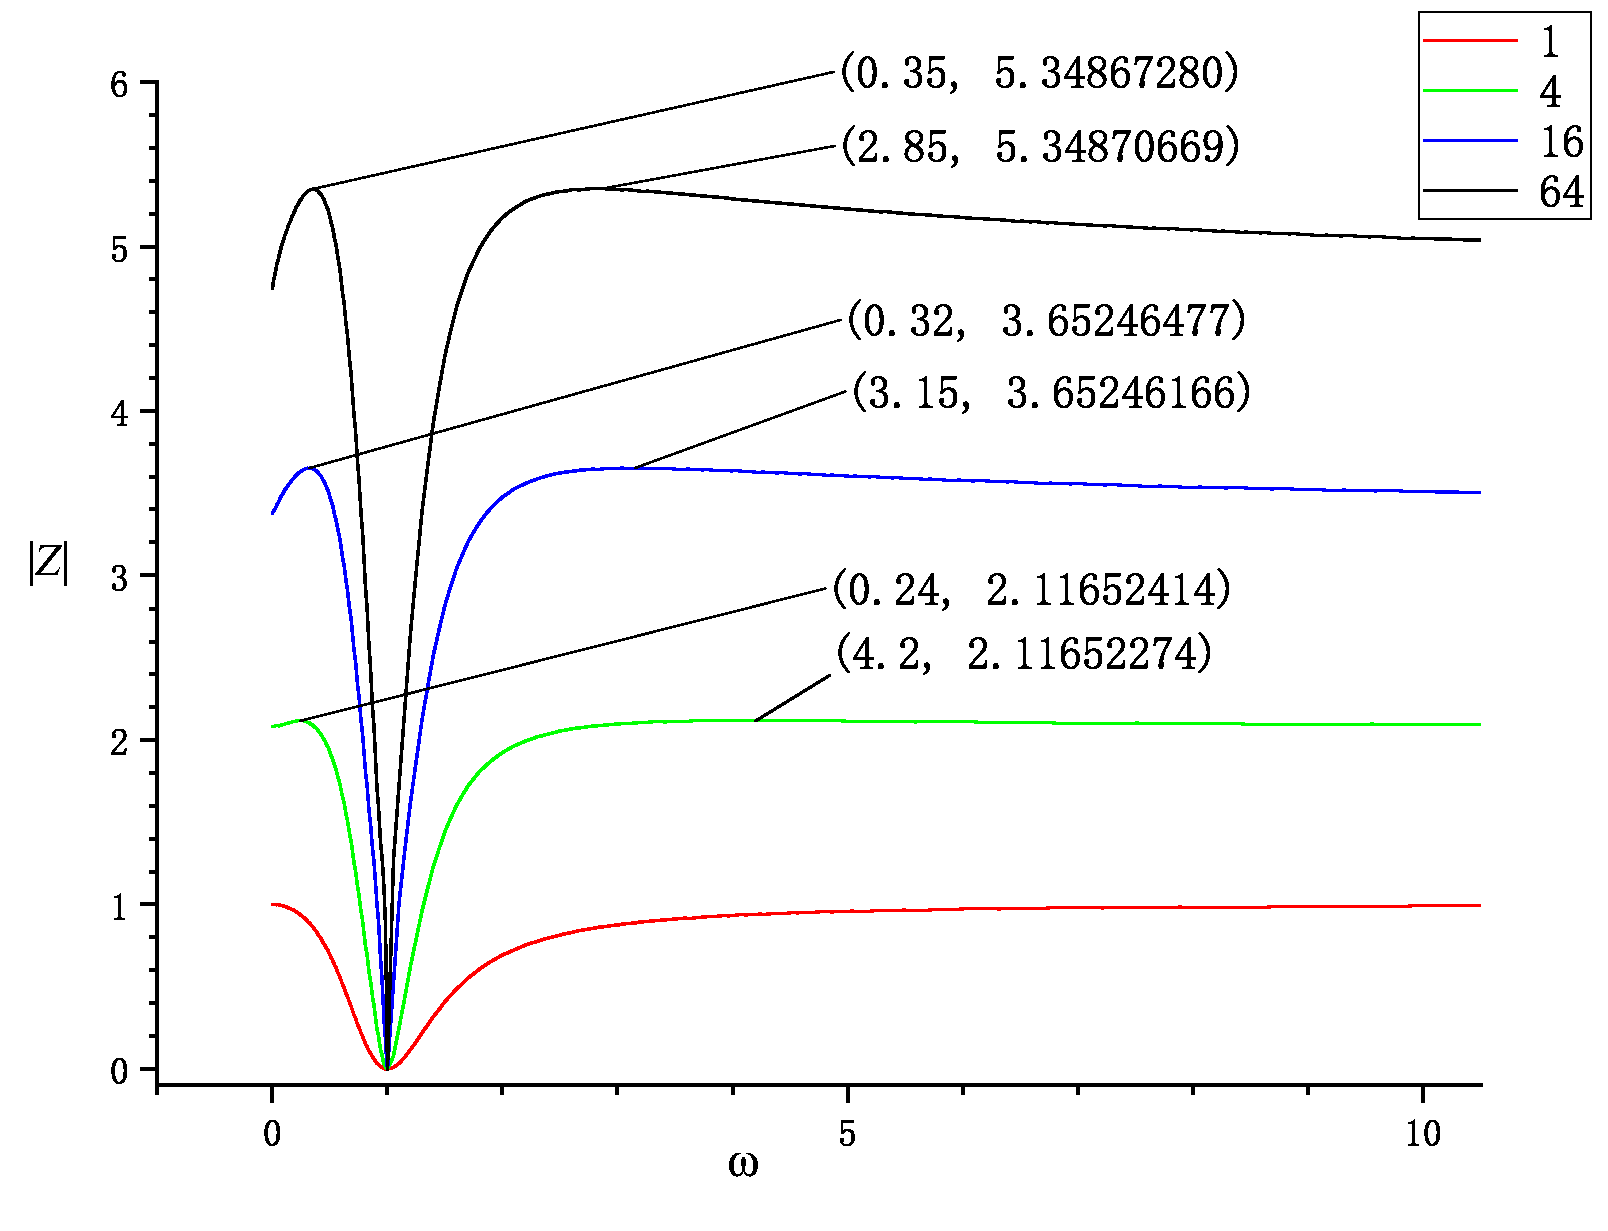
\includegraphics[width=14cm]{Abs_1_10.pdf}
            \end{center}
            \begin{center}
                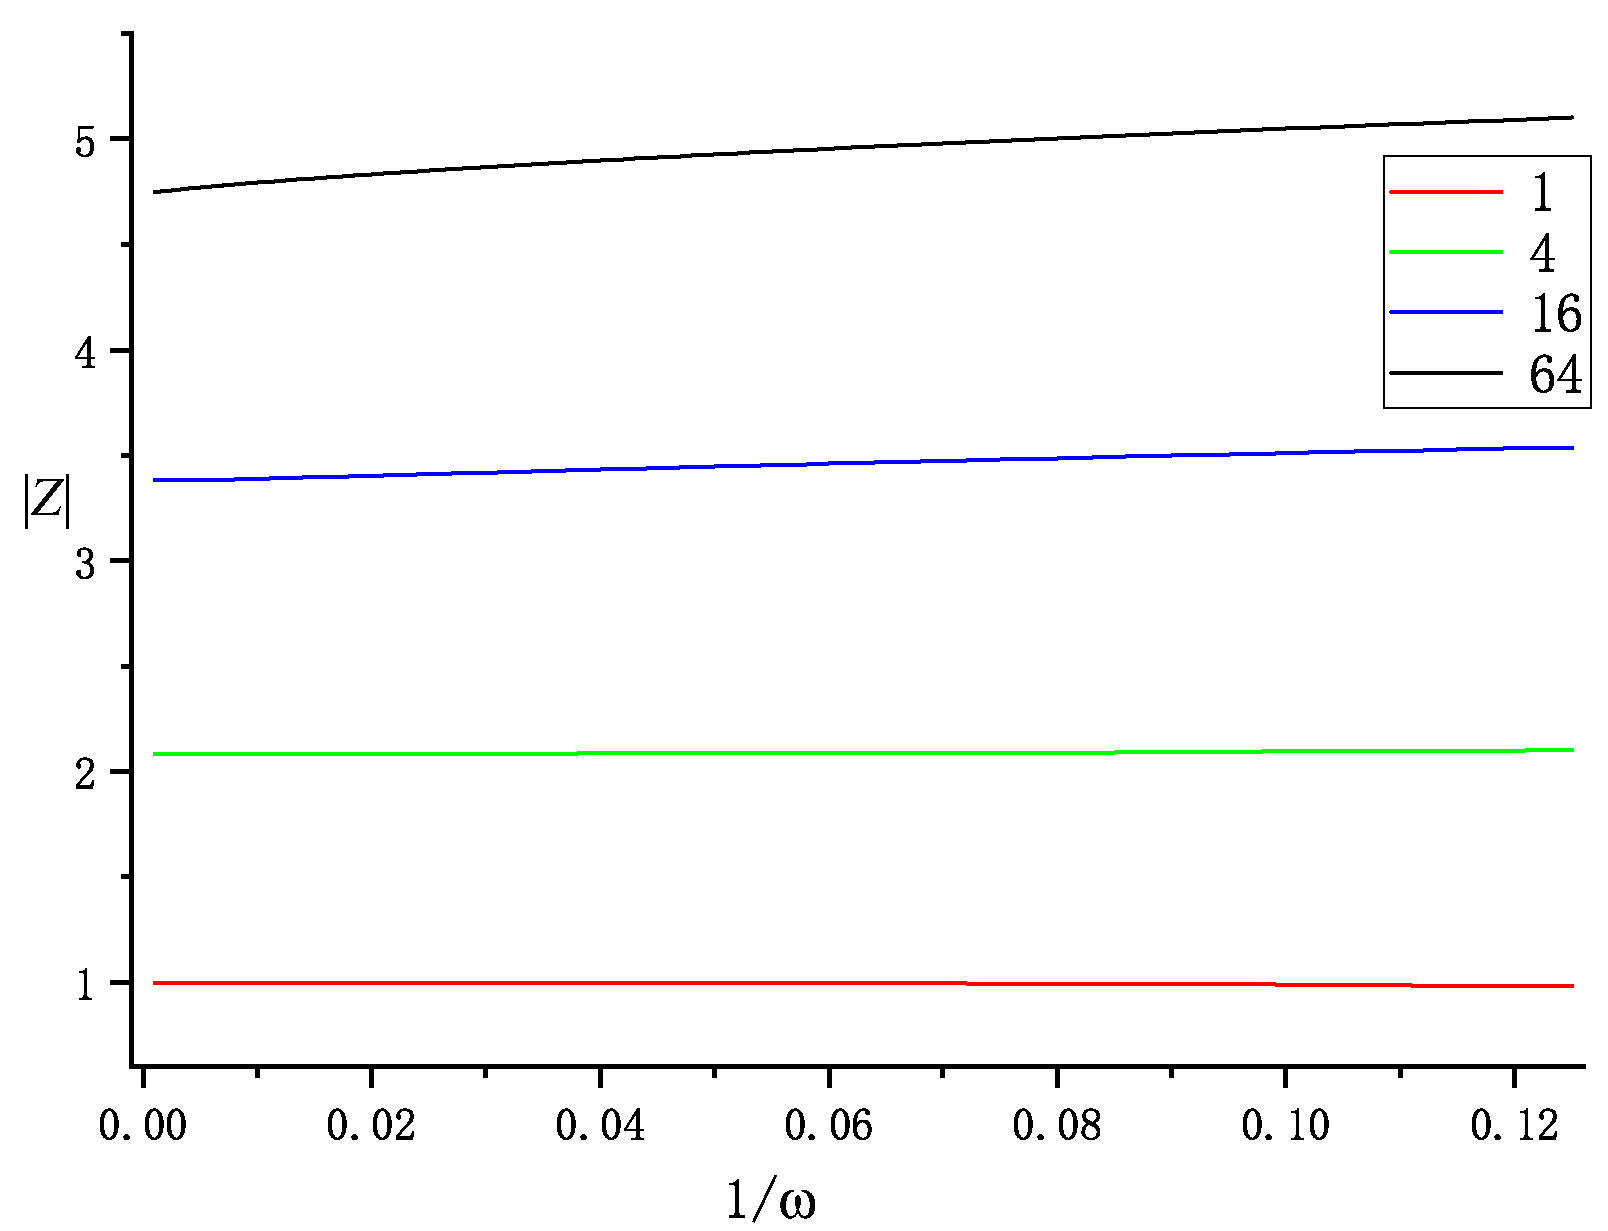
\includegraphics[width=14cm]{Abs_1000_8.pdf}
            \end{center}
            \begin{center}
                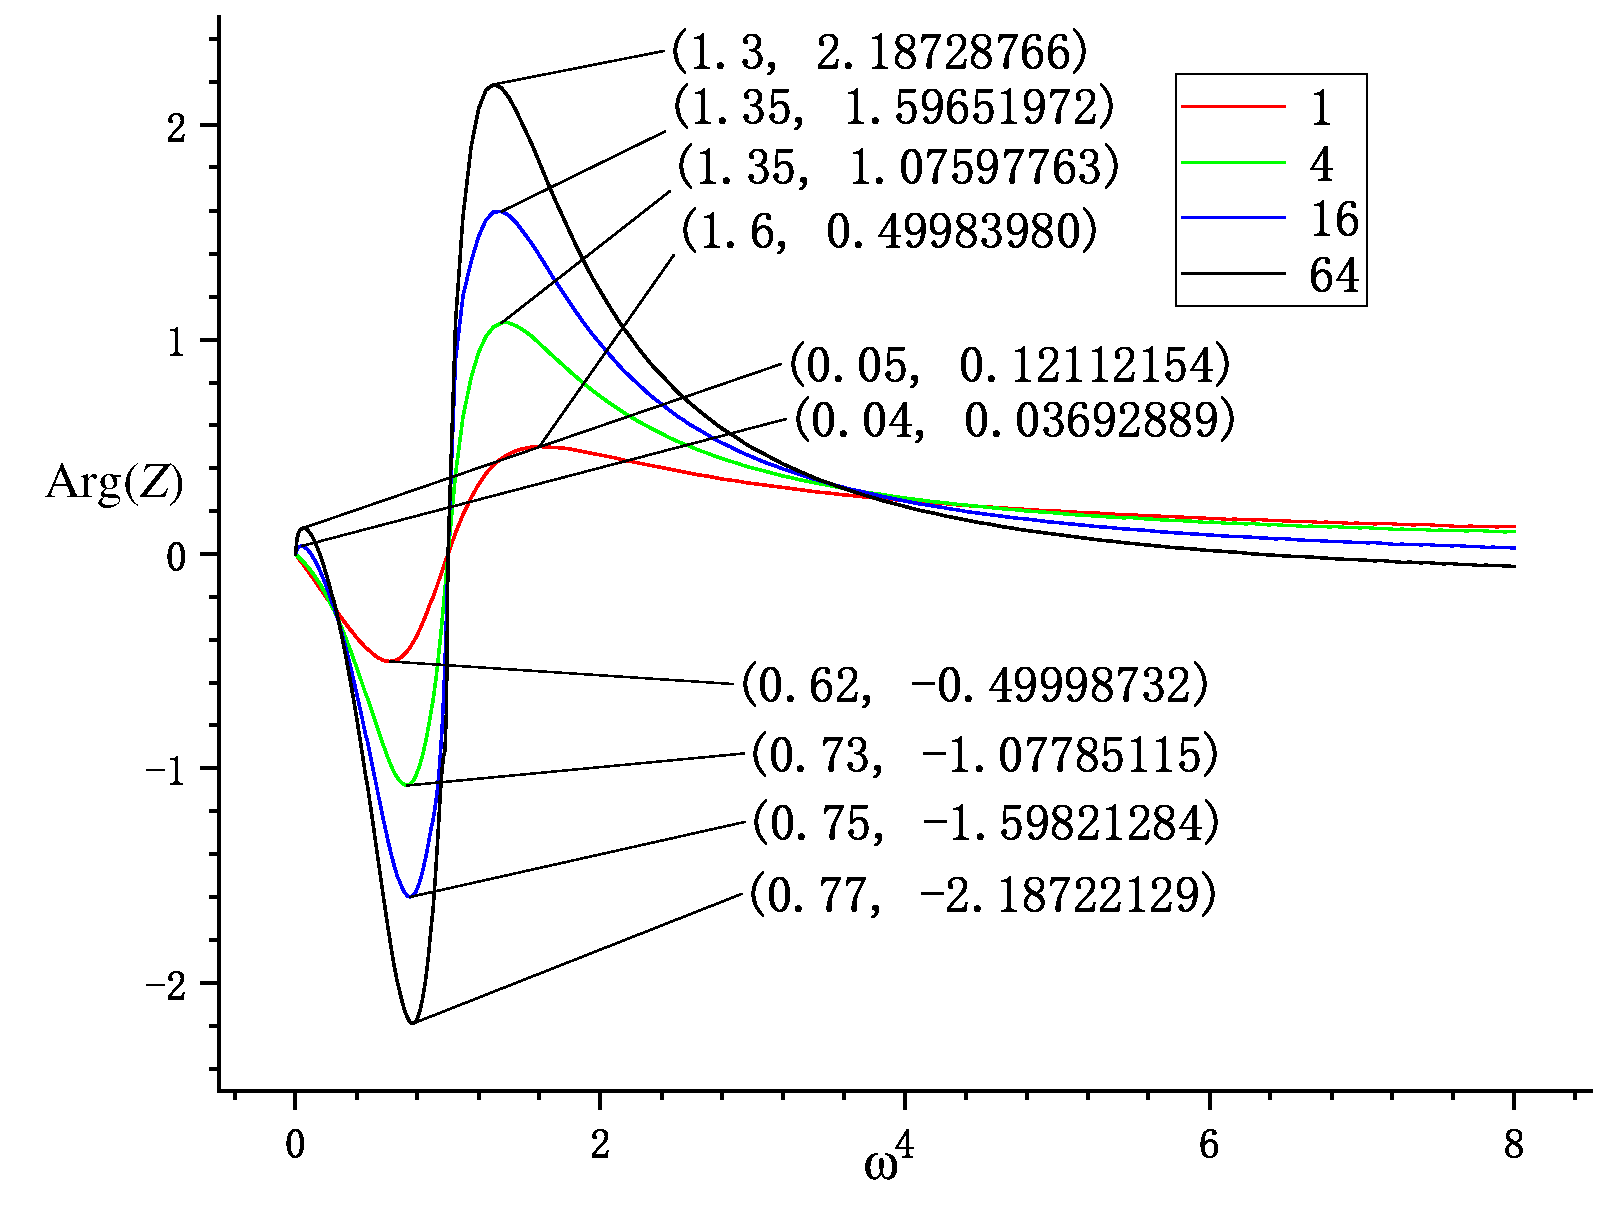
\includegraphics[width=14cm]{Arg_1_8.pdf}
            \end{center}
            \begin{center}
                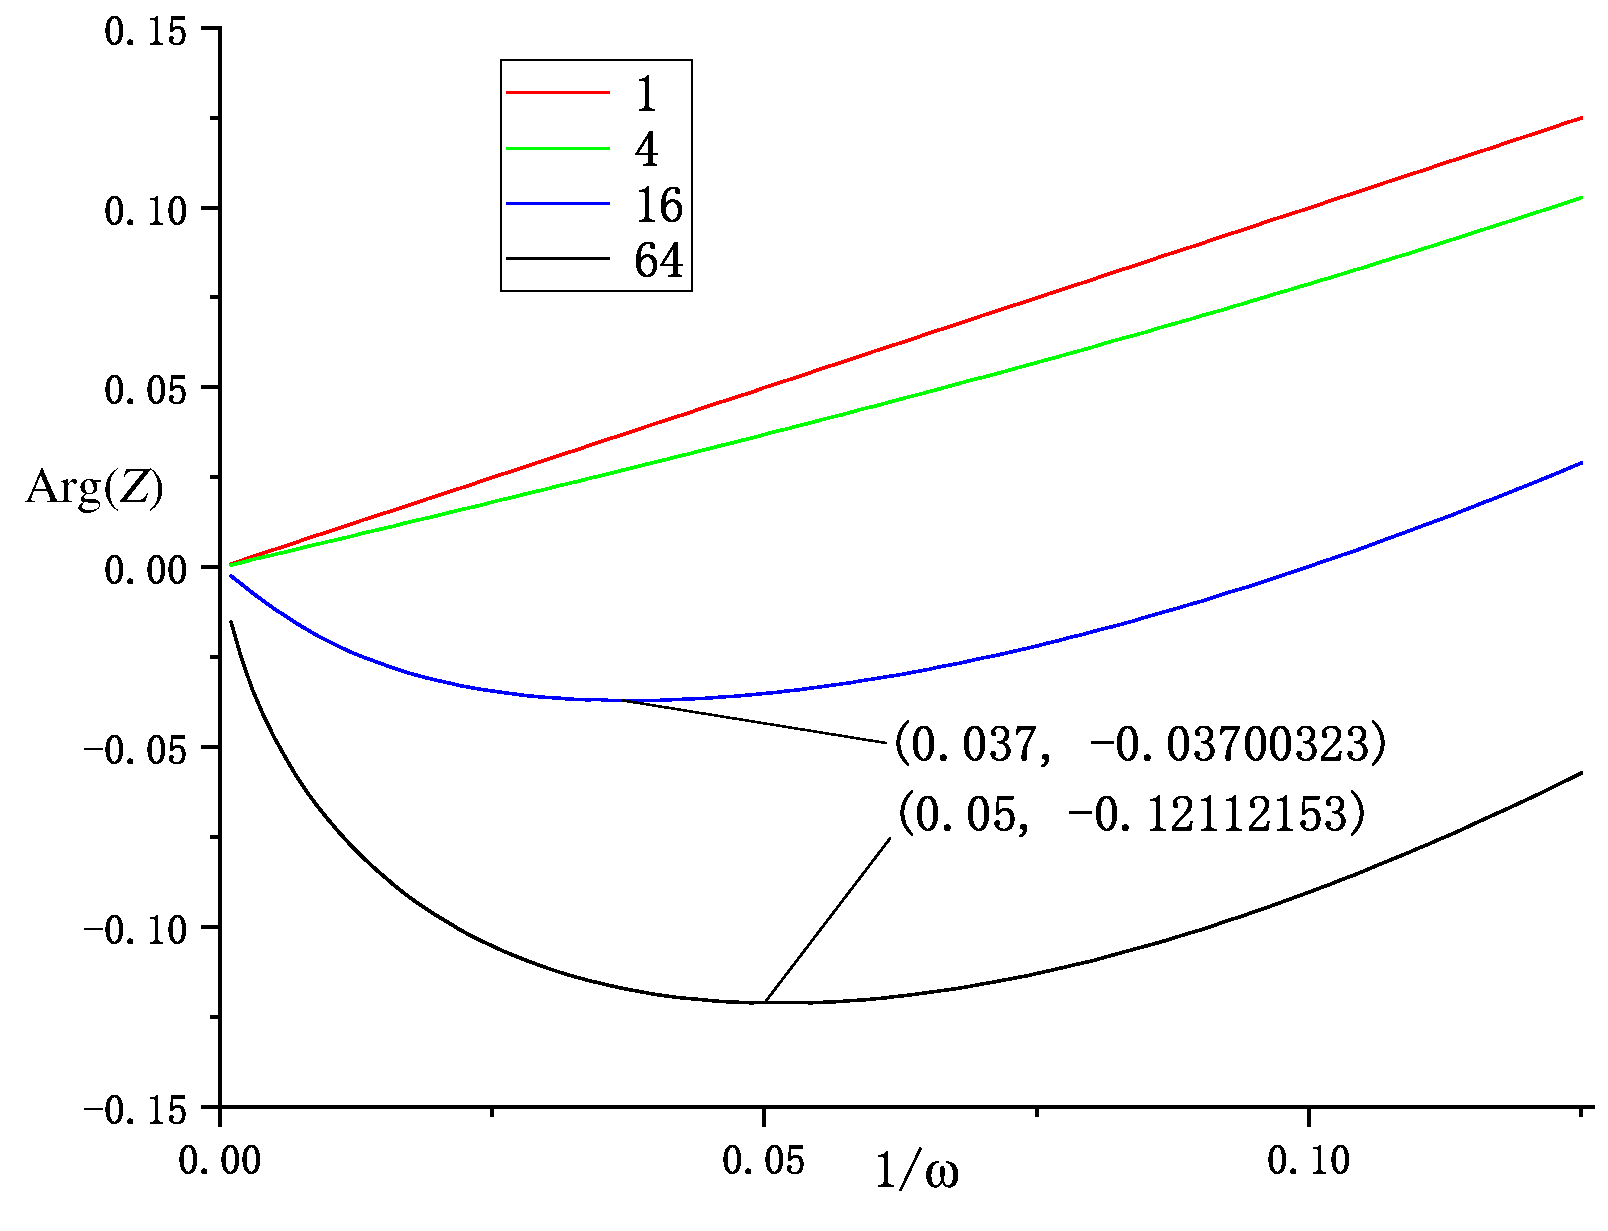
\includegraphics[width=14cm]{Arg_1000_8.pdf}
            \end{center}
            \begin{table}[H]
                \centering
                \caption{$\omega=0.5$下的耗时(CPU: Ryzen 2700x, 单线程, 仅含解方程的时间, 单位: ms)}
                \begin{tabular}{|c|c|c|c|c|c|}
                    \hline
                    规模&实矩阵分解&直接分解&实矩阵迭代&直接迭代&厄密矩阵迭代\\
                    \hline
                    1&0.006&0.008&0.065&0.054&0.051\\
                    \hline
                    4&0.011&0.007&0.135&0.310&0.081\\
                    \hline
                    16&0.232&0.090&5.217&1.015&2.889\\
                    \hline
                    64&17.647&6.433&1457.477&100k次迭代不收敛&532.640\\
                    \hline
                \end{tabular}
            \end{table}
        \subsection{直接解法-带状对称矩阵Cholesky分解法}
            \subsubsection{转换成实矩阵}
                \indent 由于n个$\mathbb{C}$上的线性方程可以写成2n个$\mathbb{R}$上的线性方程,
                所以将矩阵进行保持对称性的变形后可以直接利用之前的程序计算.
            \subsubsection{直接套用实矩阵}
                \indent 直接将原来的分解套用于复矩阵即可.
        \subsection{迭代解法-共轭梯度迭代法}
            \subsubsection{转换成实矩阵}
                \indent 同上, 转换成2n维实矩阵后直接利用原来的程序计算.
            \subsubsection{直接套用实矩阵}
                \indent 套用实矩阵的共轭梯度算法, 不改变内积形式 (不取共轭再内积)直接计算.
            \subsubsection{转换成厄密矩阵}
                \indent 把原来的内积形式改为$x^\dagger y$, 将原有的方程改写为$A^\dagger Ax=A^\dagger b$再进行迭代
                (可以通过乘2次矩阵以避免出现矩阵乘法和乘出来的稠密矩阵).
        \subsection{耗时比较}
            \indent 转换成实矩阵再分解会慢很多 (由于维数和带宽加倍), 转换成厄密矩阵的计算的结果收敛性比直接迭代或转换成实矩阵好很多.
\end{document}